
\section{Front Obstacle Detection}
To robustly detect obstacles in its forward path, the robot employs a combination of an \textbf{ultrasonic distance-measuring sensor} and \textbf{infrared (IR) proximity sensors}. A simplified representation of the obstacle detection algorithm is depicted in Fig.~\ref{fig:obstacle_diagram}.

\begin{figure} [H]
	\centering
	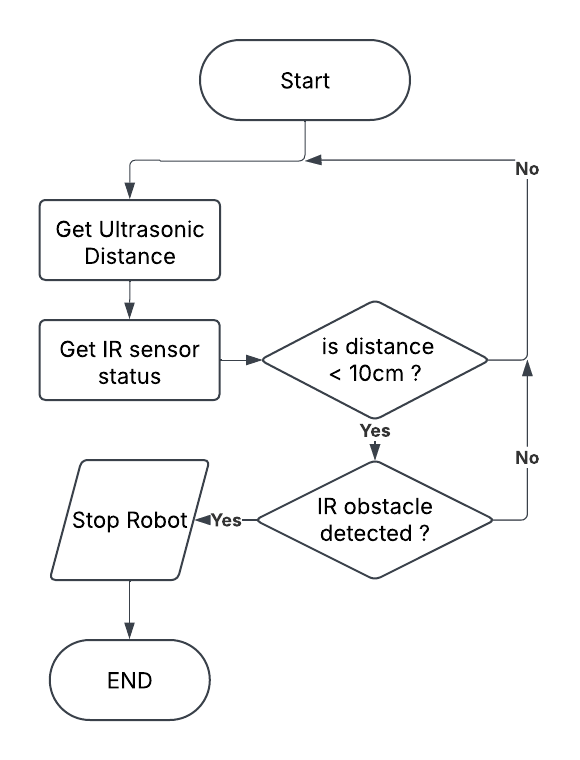
\includegraphics[height=9cm]{assets/obstacle_diagram}
	\caption{Flowchart for a robot's obstacle avoidance alogrithm using ultrasonic and infrared sensors.}
	\label{fig:obstacle_diagram}
\end{figure}


\subsubsection{Ultrasonic Distance Sensor} \label{HC-SR04}
The HC-SR04 is an ultrasonic distance sensor used for measuring the distance to an obstacle by sending an ultrasonic pulse and measuring the time it takes for the echo to return. It operates based on the principle of time-of-flight of sound waves, with a known speed of sound in air.
\begin{figure}[H]
	\centering
	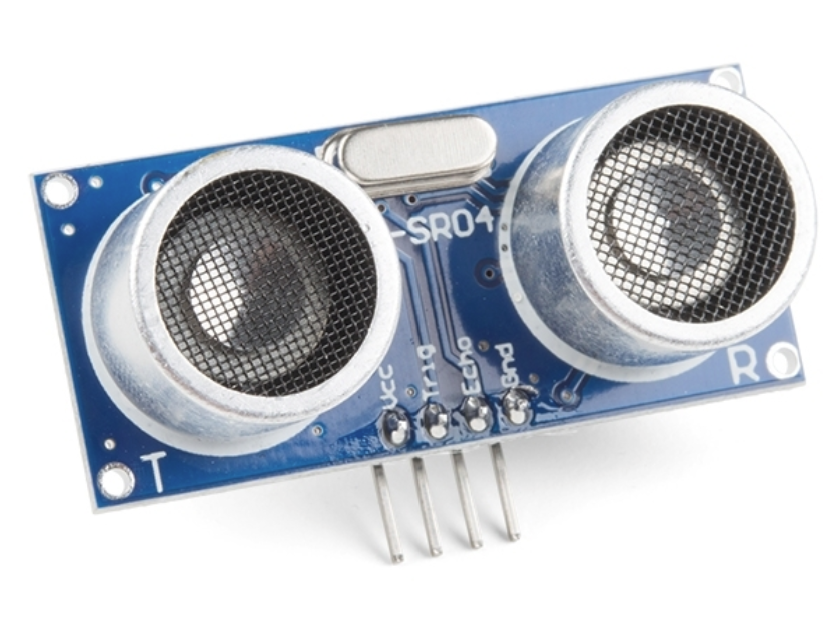
\includegraphics[width=0.25\linewidth]{assets/Ultrasonic-HC-SR04.png}
	\caption{Ultrasonic distance sensor by  Sparkfun electronics \cite{ultrasonic_sensor}.}
	\label{fig:ultra-sonic}
\end{figure}

\subsubsection{Infrared Sensing}  \label{IR_Intro}
The robot is equipped with infrared proximity sensors at the front-left and front-right directions using the Everlight Elec IR Receiver (IRM-56384) and the Infrared LED (IR204C-A). These sensors detect obstacles by transmitting a modulated infrared signal and detecting its reflection.
\begin{figure}[h]
	\centering
	\subfloat[IR204C-A \cite{ir_led}.]{
		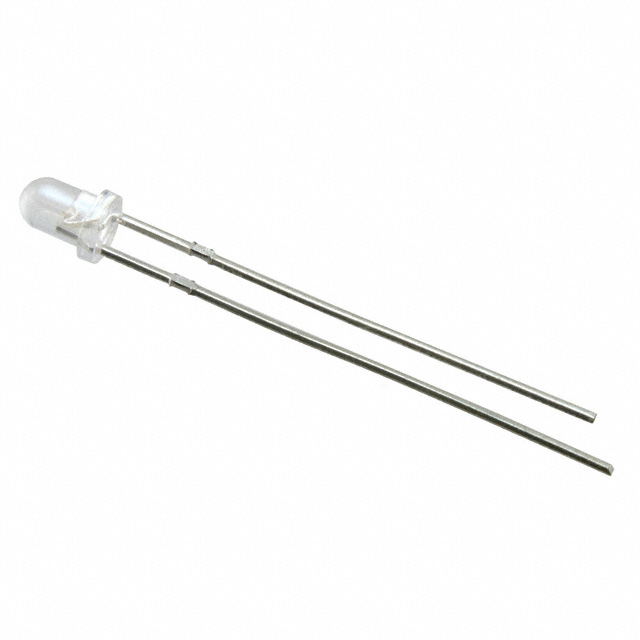
\includegraphics[height=4cm]{assets/HIR204C.jpg}
		\label{fig:ir-led}
	}
	\qquad
	\subfloat[IRM-56384 \cite{ir_receiver}.]{
		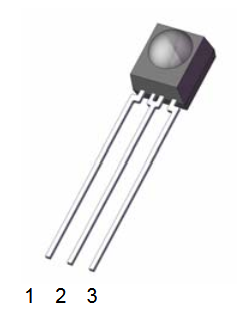
\includegraphics[height=4cm]{assets/ir-receiver.png}
		\label{fig:ir-receiver}
	}
	\caption{}
	\label{fig:ir-sensors}
\end{figure}

\subsection{Ultrasonic Working Principle}
As discussed in Section~\ref{HC-SR04}, the ultrasonic sensor operates based on the \textbf{time-of-flight} principle, utilizing sound waves to determine the distance to an obstacle. The sensor comprises two key components:
\begin{itemize}
	\item A \textbf{transmitter} that emits high-frequency ultrasonic pulses (typically at 40 kHz).
	\item A \textbf{receiver} that detects the reflected pulses after they bounce off an obstacle.
\end{itemize}

The distance to the obstacle is calculated by measuring the time delay between the transmission of the ultrasonic pulse and its reception. The formula used to compute the distance is:
\begin{equation}
	d = \frac{t \times v}{2}
\end{equation}
where:
\begin{itemize}
	\item \(d\) is the measured distance to the obstacle (in meters),
	\item \(t\) is the time delay between transmission and reception (in microseconds),
	\item \(v\) is the speed of sound in air (approximately 343 m/s at room temperature, 20°C).
\end{itemize}

\subsubsection{Ultrasonic Implementation}
The HC-SR04 requires control signals to be sent from a microcontroller:
\begin{enumerate}
	\item A short \textbf{trigger pulse} (at least 10 µs) is sent to the \texttt{TRIG} pin.
	\item The sensor responds with a high signal on the \texttt{ECHO} pin, the duration of which corresponds to the distance.
	\item The duration of the \texttt{ECHO} signal is measured to determine the distance.
\end{enumerate}

\subsubsection{Code for Distance Measurement}
Based on the datasheet \cite{ultrasonic_sensor}, an operating frequency of 20 Hz (corresponding to a 50 ms interval) is selected for distance measurements. The speed of sound is taken as 340.29 m/s, leading to the following constants in the code:

\begin{lstlisting}[style=cppstyle2]
constexpr uint8_t USONIC_GET_DISTANCE_DELAY_MS = 50; // Measurement interval
constexpr float SPEED_OF_SOUND_HALVED = (340.29 * 100.0) / (2 * 1000 * 1000); // Speed of sound in cm/us, divided by 2
\end{lstlisting}

\textbf{Code Explanation}:
\begin{itemize}
\item \texttt{USONIC\_GET\_DISTANCE\_DELAY\_MS}: Ensures measurements are taken at 20 Hz intervals.
\item \texttt{SPEED\_OF\_SOUND\_HALVED}: Converts the speed of sound to cm/µs and accounts for the round-trip travel time of the ultrasonic pulse.
\end{itemize}

The following C++ function initiates distance measurement using the HC-SR04 ultrasonic sensor:
\begin{lstlisting}[style=cppstyle2]
void StartUltrasonicMeasurement() {
	if (millis() - usonicGetDistancePrevTime > USONIC_GET_DISTANCE_DELAY_MS) {
		usonicMeasureFlag = SEND;
		usonicGetDistancePrevTime = millis(); // Update timestamp
		
		attachPinChangeInterrupt(ECHO_PIN, HandleUltrasonicMeasurementInterrupt, RISING); // Attach interrupt for rising edge
		
		digitalWrite(TRIG_PIN, LOW); 	// Reset TRIG pin
		delayMicroseconds(2);
		digitalWrite(TRIG_PIN, HIGH); 	// Send 10 us trigger pulse
		delayMicroseconds(10);
		digitalWrite(TRIG_PIN, LOW); 	// Reset TRIG pin
	}
}
\end{lstlisting}
\textbf{Code Explanation}:
\begin{itemize}
	\item The function \texttt{StartUltrasonicMeasurement()} ensures that the measurement is taken at regular intervals.
	\item A global flag \texttt{usonicMeasureFlag} is set to \texttt{SEND}, indicating that the trigger pulse is sent.
	\item The function \texttt{attachPinChangeInterrupt()} attaches an interrupt to detect when the \texttt{ECHO} pin goes HIGH.
	\item The \texttt{TRIG} pin is first set LOW (to reset), then HIGH (to trigger the pulse), and then set LOW again.
\end{itemize}
This setup enables precise distance measurement by capturing the time delay between sending and receiving the ultrasonic pulse.


\subsubsection{Interrupt Service Routine}
The following function handles the interrupt to measure the distance using the ultrasonic sensor:

\begin{lstlisting}[style=cppstyle2]
void HandleUltrasonicMeasurementInterrupt() {
	if (usonicMeasureFlag == SEND) {
		usonicMeasurePrevTime = micros();	// Record timestamp of rising edge
		attachPinChangeInterrupt(ECHO_PIN, HandleUltrasonicMeasurementInterrupt, FALLING);
		usonicMeasureFlag = RECEIVED; 	// Update flag to indicate echo reception
	} else if (usonicMeasureFlag == RECEIVED) {
		usonicDistanceValue = (uint8_t)((micros() - usonicMeasurePrevTime) * SPEED_OF_SOUND_HALVED);	// Compute distance
		usonicMeasureFlag = IDLE;	// Reset flag for next measurement
	}
}
\end{lstlisting}

\textbf{Code Explanation}:
\begin{enumerate}
	\item \textbf{Rising Edge Detection}:
	\begin{itemize}
		\item When the \texttt{ECHO} signal rises (RISING edge), the current time is recorded using \texttt{micros()}.
		\item The interrupt is reattached to detect the falling edge of the \texttt{ECHO} signal.
		\item The flag \texttt{usonicMeasureFlag} is updated to \texttt{RECEIVED} to indicate that the echo signal is being processed.
	\end{itemize}
	\item \textbf{Falling Edge Detection}:
	\begin{itemize}
		\item When the falling edge is detected, the elapsed time is computed as the difference between the current time and the previously recorded timestamp.		
		\item The distance is calculated using the formula:
		\begin{equation}
			d = \frac{ \Delta t \times v}{2}
		\end{equation}
		\item The flag \texttt{usonicMeasureFlag} is reset to \texttt{IDLE} to prepare for the next measurement cycle.
	\end{itemize}				
\end{enumerate}

\begin{itemize}
	\item When the \texttt{ECHO} signal rises (RISING edge), the timestamp is recorded using \texttt{micros()}.
	\item The interrupt is reattached to detect the falling edge of the \texttt{ECHO} signal.
	\item When the falling edge is detected, the elapsed time is computed and converted to distance using the speed of sound formula.
	\item The system resets for the next measurement by setting \texttt{usonicMeasureFlag} to \texttt{IDLE}.
\end{itemize}


\subsection{Infrared Sensing Implementation}
As discussed in Section~\ref{IR_Intro}, Infrared LED and Reciever.
The following code implements the control and processing logic for the \textbf{IR proximity sensors}:
\begin{lstlisting}[style=cppstyle2]
void IRSesorSend38KPule(unsigned char ir_pin){
	for( int i = 0; i < 39; i++) {
		digitalWrite(ir_pin, LOW);
		delayMicroseconds(9);
		digitalWrite(ir_pin, HIGH);
		delayMicroseconds(9);
	}
}

void ProcessLeftIRSensor(){
	if (millis() - irLeftCountTime > IR_COUNT_DELAY_MS) {
		UpdateSlidingWindow(irLeftPulseCount >= 3, irLeftHistory, irLeftIndex, irLeftRunningCount);    
		irLeftIsObstacle = (irLeftRunningCount >= 5); // Check if obstacle is detected
		irLeftPulseCount = 0;
		irLeftCountTime = millis(); // Update timestamp
	}
}

void ProcessRightIRSensor(){
	if (millis() - irRightCountTime > IR_COUNT_DELAY_MS) {
		UpdateSlidingWindow((irRightPulseCount >= 3), irRightHistory, irRightIndex, irRightRunningCount);
		irRightIsObstacle = (irRightRunningCount >= 5); // Check if obstacle is detected
		irRightPulseCount = 0; // Reset pulse coun
		irRightCountTime = millis(); // Update timestamp
	}
}
\end{lstlisting}

\textbf{Code Explanation}:
\begin{enumerate}
	\item \textbf{IR Pulse Generation}:
	\begin{itemize}
		\item The function \texttt{IRSensorSend38KPulse()} generates a 38 kHz modulated signal by toggling the IR LED pin at a specific frequency.
		\item Each cycle consists of 9 µs LOW and 9 µs HIGH states, repeated 39 times to ensure reliable signal transmission.
	\end{itemize}
	\item \textbf{Sensor Data Processing}:
	\begin{itemize}
		\item The functions \texttt{ProcessLeftIRSensor()} and \texttt{ProcessRightIRSensor()} process the data from the left and right IR sensors, respectively.
		\item A sliding window algorithm is used to filter out noise and improve detection reliability:
		\item The function \texttt{UpdateSlidingWindow()} updates a history buffer and running count of detected pulses. 
		\item An obstacle is considered detected if the running count exceeds a threshold (e.g., 5 out of 10 readings).
	\end{itemize}
	\item  \textbf{Obstacle Detection}:
	\begin{itemize}
		\item The flags \texttt{irLeftIsObstacle} and \texttt{irRightIsObstacle} indicate whether an obstacle is detected on the left or right side, respectively.		
		\item The pulse counts and timestamps are reset after each processing cycle to prepare for the next measurement.
	\end{itemize}
\end{enumerate}